\documentclass{beamer}
\usepackage[utf8]{inputenc}
\usepackage[T1]{fontenc}
\usepackage{graphicx}
\usepackage{xcolor}
\usepackage{tikz}
\usepackage{amsmath}
\usepackage{hyperref}
\usepackage{fontawesome}

% Theme
\usetheme{Madrid}
\usecolortheme{default}

% Colors
\definecolor{courseblue}{RGB}{0,102,204}
\definecolor{courseorange}{RGB}{255,140,0}
\definecolor{coursegreen}{RGB}{34,139,34}
\definecolor{coursered}{RGB}{220,20,60}

% Custom theme colors
\setbeamercolor{palette primary}{bg=courseblue,fg=white}
\setbeamercolor{palette secondary}{bg=courseblue!70,fg=white}
\setbeamercolor{palette tertiary}{bg=courseblue!40,fg=black}
\setbeamercolor{palette quaternary}{bg=courseblue!10,fg=black}
\setbeamercolor{structure}{fg=courseblue}
\setbeamercolor{frametitle}{bg=courseblue,fg=white}

% Title page info
\title{C Programming for Post-Silicon Validation Engineers}
\subtitle{6-Day Intensive Bootcamp}
\author{Training Program Proposal}
\date{2025}
\institute{Professional Development Initiative}

\begin{document}

\frame{\titlepage}

\begin{frame}
\frametitle{The Challenge: Skills Gap in Validation Engineering}

\begin{columns}
\begin{column}{0.5\textwidth}
\textbf{Industry Reality:}
\begin{itemize}
    \item Post-silicon validation is critical for chip success
    \item Engineers need C programming for validation tools
    \item Most engineers lack embedded programming skills
    \item Traditional training takes months
\end{itemize}
\end{column}
\begin{column}{0.5\textwidth}
\begin{center}
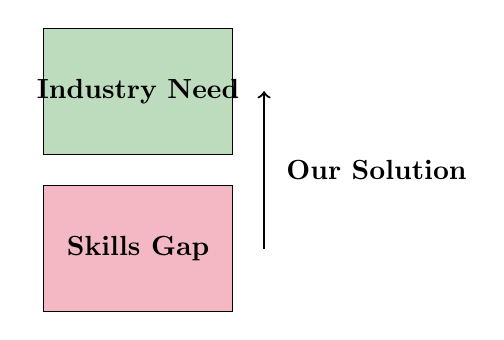
\begin{tikzpicture}[scale=0.8]
% Skills gap visualization
\draw[fill=coursered!30] (0,0) rectangle (3,2);
\node at (1.5,1) {\textbf{Skills Gap}};

\draw[fill=coursegreen!30] (0,2.5) rectangle (3,4.5);
\node at (1.5,3.5) {\textbf{Industry Need}};

\draw[thick,->] (3.5,1) -- (3.5,3.5);
\node[right] at (3.7,2.25) {\textbf{Our Solution}};
\end{tikzpicture}
\end{center}
\end{column}
\end{columns}

\vspace{0.5cm}
\begin{alertblock}{The Problem}
Engineers with semiconductor knowledge but no programming experience need rapid upskilling for validation roles.
\end{alertblock}
\end{frame}

\begin{frame}
\frametitle{Our Solution: Intensive C Programming Bootcamp}

\begin{center}
\Large \textbf{From Zero to Validation Hero in 6 Days}
\end{center}

\vspace{0.5cm}

\begin{columns}
\begin{column}{0.6\textwidth}
\textbf{Key Features:}
\begin{itemize}
    \item \textcolor{courseblue}{\textbf{Validation-Focused:}} All examples simulate real post-silicon scenarios
    \item \textcolor{courseblue}{\textbf{Hands-On:}} 60\% lab time with real RP2040 hardware
    \item \textcolor{courseblue}{\textbf{Progressive:}} From basic syntax to embedded systems
    \item \textcolor{courseblue}{\textbf{Modern:}} AI tools integration and GitHub workflows
    \item \textcolor{courseblue}{\textbf{Practical:}} Portfolio-ready projects
\end{itemize}
\end{column}
\begin{column}{0.4\textwidth}
\begin{center}
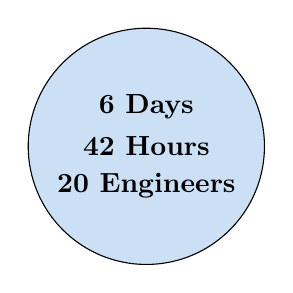
\begin{tikzpicture}
\draw[fill=courseblue!20] (0,0) circle (1.5);
\node at (0,0.5) {\textbf{6 Days}};
\node at (0,0) {\textbf{42 Hours}};
\node at (0,-0.5) {\textbf{20 Engineers}};
\end{tikzpicture}
\end{center}
\end{column}
\end{columns}

\vspace{0.5cm}
\begin{exampleblock}{Unique Value Proposition}
The only course that combines C programming fundamentals with embedded validation engineering in an intensive, practical format.
\end{exampleblock}
\end{frame}

\begin{frame}
\frametitle{Target Audience and Market Need}

\begin{columns}
\begin{column}{0.5\textwidth}
\textbf{Primary Audience:}
\begin{itemize}
    \item Hardware engineers transitioning to validation
    \item Test engineers needing programming skills
    \item New graduates entering semiconductor industry
    \item Experienced engineers upskilling for modern validation
\end{itemize}

\vspace{0.5cm}
\textbf{Prerequisites:}
\begin{itemize}
    \item Basic understanding of digital electronics
    \item No programming experience required
    \item Engineering or technical background
    \item Commitment to intensive learning
\end{itemize}
\end{column}
\begin{column}{0.5\textwidth}
\textbf{Market Demand:}
\begin{center}
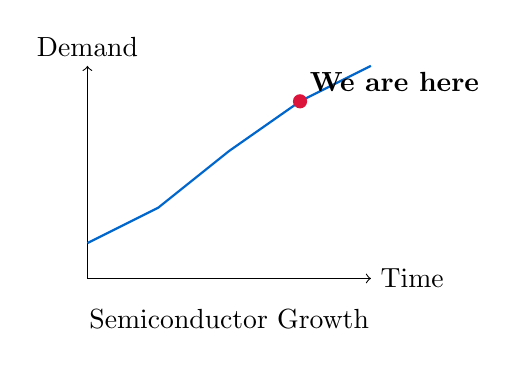
\begin{tikzpicture}[scale=0.9]
% Market demand chart
\draw[->] (0,0) -- (0,3) node[above] {Demand};
\draw[->] (0,0) -- (4,0) node[right] {Time};

\draw[thick,courseblue] (0,0.5) -- (1,1) -- (2,1.8) -- (3,2.5) -- (4,3);
\node[below] at (2,-0.3) {Semiconductor Growth};

\fill[coursered] (3,2.5) circle (0.1);
\node[above right] at (3,2.5) {\textbf{We are here}};
\end{tikzpicture}
\end{center}

\textbf{Industry Statistics:}
\begin{itemize}
    \item 73\% of validation teams report skills gaps
    \item Average time to productivity: 6-12 months
    \item Our solution: 6 days + 4 weeks mentoring
\end{itemize}
\end{column}
\end{columns}
\end{frame}

\begin{frame}
\frametitle{Curriculum Overview: 6-Day Journey}

\begin{center}
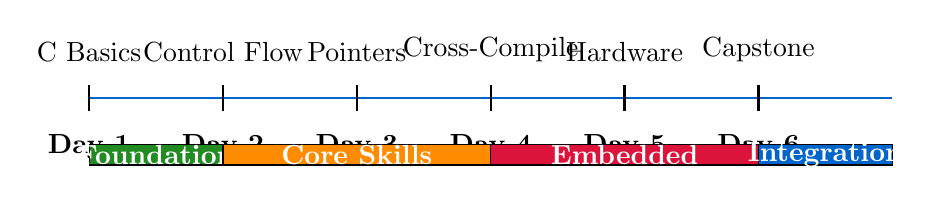
\begin{tikzpicture}[scale=0.85]
% Timeline
\draw[thick,courseblue] (0,0) -- (12,0);

% Day markers
\foreach \x/\day/\topic in {0/Day 1/C Basics, 2/Day 2/Control Flow, 4/Day 3/Pointers, 6/Day 4/Cross-Compile, 8/Day 5/Hardware, 10/Day 6/Capstone} {
    \draw[thick] (\x,-0.2) -- (\x,0.2);
    \node[below] at (\x,-0.4) {\textbf{\day}};
    \node[above] at (\x,0.4) {\topic};
}

% Progress indicators
\draw[fill=coursegreen] (0,-1) rectangle (2,-0.7);
\node at (1,-0.85) {\textcolor{white}{\textbf{Foundation}}};

\draw[fill=courseorange] (2,-1) rectangle (6,-0.7);
\node at (4,-0.85) {\textcolor{white}{\textbf{Core Skills}}};

\draw[fill=coursered] (6,-1) rectangle (10,-0.7);
\node at (8,-0.85) {\textcolor{white}{\textbf{Embedded}}};

\draw[fill=courseblue] (10,-1) rectangle (12,-0.7);
\node at (11,-0.85) {\textcolor{white}{\textbf{Integration}}};
\end{tikzpicture}
\end{center}

\vspace{0.5cm}

\begin{columns}
\begin{column}{0.5\textwidth}
\textbf{Learning Progression:}
\begin{itemize}
    \item \textbf{Days 1-2:} C fundamentals, debugging
    \item \textbf{Day 3:} Memory management, AI tools
    \item \textbf{Day 4:} Cross-compilation, RP2040
    \item \textbf{Day 5:} Hardware validation
    \item \textbf{Day 6:} Capstone project
\end{itemize}
\end{column}
\begin{column}{0.5\textwidth}
\textbf{Validation Focus:}
\begin{itemize}
    \item Register monitoring systems
    \item Fault injection testing
    \item Hardware-in-the-loop validation
    \item Performance optimization
    \item Professional documentation
\end{itemize}
\end{column}
\end{columns}
\end{frame>

\begin{frame}
\frametitle{Hands-On Learning with Real Hardware}

\begin{columns}
\begin{column}{0.6\textwidth}
\textbf{RP2040 Platform Benefits:}
\begin{itemize}
    \item \textcolor{courseblue}{\textbf{Real ARM Cortex-M0+:}} Industry-standard architecture
    \item \textcolor{courseblue}{\textbf{Low Cost:}} \$4-5 per board, scalable program
    \item \textcolor{courseblue}{\textbf{Easy Programming:}} USB drag-and-drop flashing
    \item \textcolor{courseblue}{\textbf{Rich Peripherals:}} GPIO, ADC, timers, communication
    \item \textcolor{courseblue}{\textbf{Excellent Documentation:}} Comprehensive SDK and examples
\end{itemize>

\vspace{0.5cm}
\textbf{Validation Applications:}
\begin{itemize}
    \item Multi-peripheral testing suites
    \item Real-time constraint validation
    \item Fault injection and recovery
    \item Performance benchmarking
\end{itemize>
\end{column>
\begin{column}{0.4\textwidth}
\begin{center}
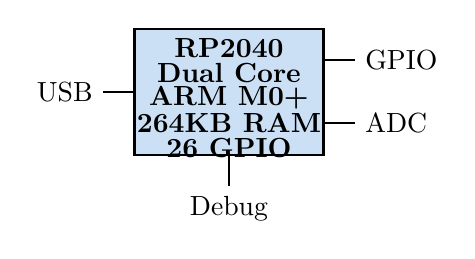
\begin{tikzpicture}[scale=0.8]
% RP2040 representation
\draw[fill=courseblue!20, thick] (0,0) rectangle (3,2);
\node at (1.5,1.7) {\textbf{RP2040}};
\node at (1.5,1.3) {\textbf{Dual Core}};
\node at (1.5,0.9) {\textbf{ARM M0+}};
\node at (1.5,0.5) {\textbf{264KB RAM}};
\node at (1.5,0.1) {\textbf{26 GPIO}};

% Connections
\draw[thick] (0,1) -- (-0.5,1) node[left] {USB};
\draw[thick] (3,1.5) -- (3.5,1.5) node[right] {GPIO};
\draw[thick] (3,0.5) -- (3.5,0.5) node[right] {ADC};
\draw[thick] (1.5,0) -- (1.5,-0.5) node[below] {Debug};
\end{tikzpicture}
\end{center>

\vspace{0.5cm}
\textbf{Hardware Budget:}
\begin{itemize}
    \item 20 RP2040 boards: \$100
    \item USB cables: \$30
    \item Accessories: \$20
    \item \textbf{Total: \$150}
\end{itemize>
\end{column>
\end{columns>
\end{frame>

\begin{frame}
\frametitle{Modern Development Practices}

\begin{columns}
\begin{column}{0.5\textwidth}
\textbf{Professional Toolchain:}
\begin{itemize}
    \item \textbf{GCC:} Industry-standard C compiler
    \item \textbf{GDB:} Professional debugging tools
    \item \textbf{CMake:} Modern build system management
    \item \textbf{VS Code:} Popular development environment
    \item \textbf{GitHub:} Version control and collaboration
\end{itemize}

\vspace{0.5cm}
\textbf{AI Integration:}
\begin{itemize}
    \item Responsible AI tool usage (Day 3+)
    \item Critical evaluation of AI suggestions
    \item Documentation requirements
    \item Balance of AI assistance with learning
\end{itemize}
\end{column}
\begin{column}{0.5\textwidth}
\begin{center}
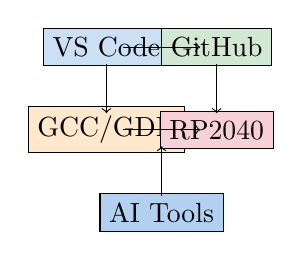
\begin{tikzpicture}[scale=0.7]
% Development workflow
\node[draw, rectangle, fill=courseblue!20] at (0,3) {VS Code};
\node[draw, rectangle, fill=coursegreen!20] at (2,3) {GitHub};
\node[draw, rectangle, fill=courseorange!20] at (0,1.5) {GCC/GDB};
\node[draw, rectangle, fill=coursered!20] at (2,1.5) {RP2040};
\node[draw, rectangle, fill=courseblue!30] at (1,0) {AI Tools};

% Connections
\draw[->] (0,2.7) -- (0,1.8);
\draw[->] (0.3,3) -- (1.7,3);
\draw[->] (2,2.7) -- (2,1.8);
\draw[->] (0.3,1.5) -- (1.7,1.5);
\draw[->] (1,0.3) -- (1,1.2);
\end{tikzpicture}
\end{center>

\textbf{Portfolio Development:}
\begin{itemize}
    \item Professional GitHub repositories
    \item Documented validation projects
    \item Technical presentation skills
    \item Industry-ready code samples
\end{itemize>
\end{column>
\end{columns>

\begin{exampleblock}{Career Readiness}
Graduates leave with a professional portfolio demonstrating embedded validation skills to potential employers.
\end{exampleblock>
\end{frame>

\begin{frame}
\frametitle{Assessment and Quality Assurance}

\begin{columns}
\begin{column}{0.5\textwidth}
\textbf{Comprehensive Evaluation:}
\begin{itemize}
    \item \textbf{35\%} Daily lab assignments (auto-graded)
    \item \textbf{35\%} Capstone project (team-based)
    \item \textbf{30\%} Participation and collaboration
\end{itemize}

\vspace{0.5cm}
\textbf{GitHub Classroom Integration:}
\begin{itemize}
    \item Automated compilation testing
    \item Unit test execution
    \item Code quality analysis
    \item Progress tracking
    \item Plagiarism detection
\end{itemize}
\end{column}
\begin{column}{0.5\textwidth}
\textbf{Success Metrics:}
\begin{center}
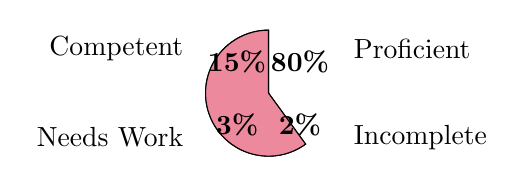
\begin{tikzpicture}[scale=0.8]
% Success metrics pie chart
\draw[fill=coursegreen!50] (0,0) -- (0,1) arc (90:162:1) -- cycle;
\draw[fill=courseblue!50] (0,0) -- (162:1) arc (162:234:1) -- cycle;
\draw[fill=courseorange!50] (0,0) -- (234:1) arc (234:306:1) -- cycle;
\draw[fill=coursered!50] (0,0) -- (306:1) arc (306:90:1) -- cycle;

\node at (0.5,0.5) {\textbf{80\%}};
\node at (-0.5,0.5) {\textbf{15\%}};
\node at (-0.5,-0.5) {\textbf{3\%}};
\node at (0.5,-0.5) {\textbf{2\%}};

\node[right] at (1.2,0.7) {Proficient};
\node[left] at (-1.2,0.7) {Competent};
\node[left] at (-1.2,-0.7) {Needs Work};
\node[right] at (1.2,-0.7) {Incomplete};
\end{tikzpicture}
\end{center>

\textbf{Quality Indicators:}
\begin{itemize}
    \item Pre/post skill assessments
    \item Portfolio quality reviews
    \item Employer feedback (6 months)
    \item Alumni career progression
\end{itemize>
\end{column>
\end{columns>

\begin{alertblock}{Target: 80\%+ Proficiency Rate}
Based on pilot programs and similar intensive bootcamps in the industry.
\end{alertblock>
\end{frame>

\begin{frame}
\frametitle{Implementation Plan and Timeline}

\begin{columns}
\begin{column}{0.6\textwidth}
\textbf{Phase 1: Preparation (4 weeks)}
\begin{itemize}
    \item Instructor training and certification
    \item Hardware procurement and testing
    \item GitHub Classroom setup
    \item Marketing and participant recruitment
\end{itemize}

\textbf{Phase 2: Pilot Program (1 week)}
\begin{itemize}
    \item First cohort of 20 engineers
    \item Intensive feedback collection
    \item Curriculum refinement
    \item Process optimization
\end{itemize>

\textbf{Phase 3: Scale-Up (Ongoing)}
\begin{itemize}
    \item Monthly cohorts of 20 participants
    \item Advanced modules development
    \item Corporate partnership programs
    \item Train-the-trainer expansion
\end{itemize>
\end{column}
\begin{column}{0.4\textwidth}
\begin{center}
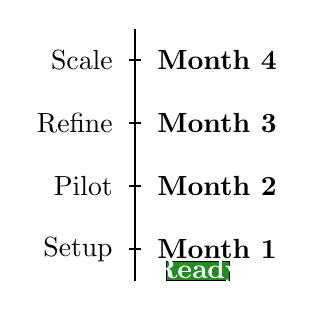
\begin{tikzpicture}[scale=0.8]
% Timeline
\draw[thick] (0,0) -- (0,4);

% Milestones
\foreach \y/\month/\milestone in {0.5/Month 1/Setup, 1.5/Month 2/Pilot, 2.5/Month 3/Refine, 3.5/Month 4/Scale} {
    \draw[thick] (-0.1,\y) -- (0.1,\y);
    \node[right] at (0.2,\y) {\textbf{\month}};
    \node[left] at (-0.2,\y) {\milestone};
}

% Success indicators
\draw[fill=coursegreen] (0.5,0) rectangle (1.5,0.3);
\node at (1,0.15) {\textcolor{white}{\textbf{Ready}}};
\end{tikzpicture}
\end{center>

\textbf{Scalability Features:}
\begin{itemize}
    \item Standardized curriculum
    \item Automated assessment
    \item Reusable hardware kits
    \item Remote delivery options
    \item Corporate customization
\end{itemize>
\end{column>
\end{columns>

\vspace{0.5cm}
\begin{exampleblock}{Rapid Deployment}
Program can be launched within 4 weeks of approval, with first cohort graduating in 6 weeks.
\end{exampleblock>
\end{frame>

\begin{frame}
\frametitle{Budget and Resource Requirements}

\begin{columns}
\begin{column}{0.5\textwidth}
\textbf{One-Time Setup Costs:}
\begin{itemize}
    \item Hardware (20 RP2040 kits): \$150
    \item Curriculum development: \$5,000
    \item Instructor training: \$2,000
    \item Platform setup: \$1,000
    \item \textbf{Total Setup: \$8,150}
\end{itemize}

\vspace{0.5cm}
\textbf{Per-Cohort Operating Costs:}
\begin{itemize}
    \item Instructor (1 week): \$3,000
    \item Teaching assistants (2): \$1,000
    \item Materials and supplies: \$200
    \item Facility and equipment: \$500
    \item \textbf{Total per Cohort: \$4,700}
\end{itemize}
\end{column>
\begin{column}{0.5\textwidth}
\textbf{Revenue Model:}
\begin{center}
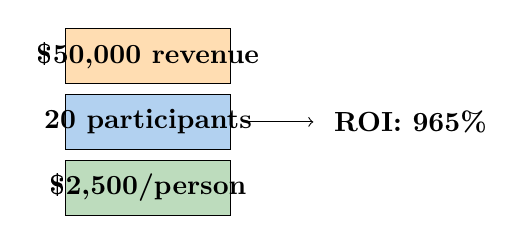
\begin{tikzpicture}[scale=0.7]
% Revenue breakdown
\draw[fill=coursegreen!30] (0,0) rectangle (3,1);
\node at (1.5,0.5) {\textbf{\$2,500/person}};

\draw[fill=courseblue!30] (0,1.2) rectangle (3,2.2);
\node at (1.5,1.7) {\textbf{20 participants}};

\draw[fill=courseorange!30] (0,2.4) rectangle (3,3.4);
\node at (1.5,2.9) {\textbf{\$50,000 revenue}};

\draw[->] (3.2,1.7) -- (4.5,1.7);
\node[right] at (4.7,1.7) {\textbf{ROI: 965\%}};
\end{tikzpicture}
\end{center>

\textbf{Break-Even Analysis:}
\begin{itemize}
    \item Revenue per cohort: \$50,000
    \item Costs per cohort: \$4,700
    \item Profit per cohort: \$45,300
    \item Break-even: 1 cohort
\end{itemize>

\textbf{Annual Projections:}
\begin{itemize}
    \item 12 cohorts/year: 240 engineers
    \item Annual revenue: \$600,000
    \item Annual profit: \$543,600
\end{itemize>
\end{column>
\end{columns>
\end{frame>

\begin{frame}
\frametitle{Competitive Advantages and Differentiation}

\begin{columns}
\begin{column}{0.5\textwidth}
\textbf{Unique Positioning:}
\begin{itemize}
    \item \textcolor{courseblue}{\textbf{Validation-Specific:}} Only course focused on post-silicon validation
    \item \textcolor{courseblue}{\textbf{Intensive Format:}} 6 days vs. months of traditional training
    \item \textcolor{courseblue}{\textbf{Real Hardware:}} Hands-on RP2040 experience
    \item \textcolor{courseblue}{\textbf{Modern Tools:}} AI integration and GitHub workflows
    \item \textcolor{courseblue}{\textbf{Portfolio Focus:}} Career-ready deliverables
\end{itemize>

\vspace{0.5cm}
\textbf{Competitive Landscape:}
\begin{itemize}
    \item University courses: Too theoretical, too slow
    \item Online tutorials: No validation focus, no mentoring
    \item Corporate training: Generic, expensive, lengthy
    \item Bootcamps: Web/mobile focus, not embedded
\end{itemize>
\end{column>
\begin{column}{0.5\textwidth}
\begin{center}
\begin{tikzpicture}[scale=0.8]
% Competitive positioning
\draw[->] (0,0) -- (4,0) node[right] {Speed};
\draw[->] (0,0) -- (0,4) node[above] {Relevance};

% Competitors
\fill[coursered] (1,1) circle (0.1);
\node[below] at (1,0.8) {Universities};

\fill[courseorange] (2,0.5) circle (0.1);
\node[below] at (2,0.3) {Online};

\fill[coursegreen] (0.5,2) circle (0.1);
\node[left] at (0.3,2) {Corporate};

% Our solution
\fill[courseblue] (3.5,3.5) circle (0.15);
\node[above right] at (3.5,3.5) {\textbf{Our Solution}};

% Quadrants
\draw[dashed, gray] (2,0) -- (2,4);
\draw[dashed, gray] (0,2) -- (4,2);
\end{tikzpicture>
\end{center>

\textbf{Success Factors:}
\begin{itemize}
    \item Industry-experienced instructors
    \item Proven curriculum methodology
    \item Strong industry partnerships
    \item Continuous improvement process
    \item Alumni success tracking
\end{itemize>
\end{column>
\end{columns>

\begin{exampleblock}{Market Opportunity}
First-mover advantage in validation-specific programming education with potential for industry standard adoption.
\end{exampleblock>
\end{frame>

\begin{frame}
\frametitle{Call to Action and Next Steps}

\begin{center}
\Large \textbf{Transform Your Engineering Team in 6 Days}
\end{center>

\vspace{0.5cm}

\begin{columns}
\begin{column}{0.5\textwidth}
\textbf{Immediate Benefits:}
\begin{itemize}
    \item \textcolor{coursegreen}{\textbf{Rapid Skill Development:}} 6 days vs. 6 months
    \item \textcolor{coursegreen}{\textbf{Practical Skills:}} Immediately applicable to validation work
    \item \textcolor{coursegreen}{\textbf{Team Building:}} Cohort-based collaborative learning
    \item \textcolor{coursegreen}{\textbf{Modern Practices:}} AI tools and GitHub workflows
    \item \textcolor{coursegreen}{\textbf{Portfolio Development:}} Career advancement ready
\end{itemize>

\vspace{0.5cm}
\textbf{Long-Term Impact:}
\begin{itemize}
    \item Reduced time-to-productivity for new hires
    \item Enhanced validation team capabilities
    \item Improved product quality and time-to-market
    \item Competitive advantage in validation expertise
\end{itemize>
\end{column>
\begin{column}{0.5\textwidth}
\textbf{Next Steps:}
\begin{enumerate}
    \item \textbf{Approval:} Green-light the program
    \item \textbf{Planning:} 2-week detailed planning phase
    \item \textbf{Setup:} 4-week preparation and setup
    \item \textbf{Launch:} First cohort delivery
    \item \textbf{Scale:} Monthly cohort schedule
\end{enumerate>

\vspace{0.5cm}
\begin{center}
\begin{tikzpicture}
\draw[fill=courseblue!20, thick] (0,0) rectangle (3,1.5);
\node at (1.5,0.75) {\textbf{Ready to Start}};
\node at (1.5,0.25) {\textbf{in 6 Weeks}};
\end{tikzpicture}
\end{center>

\textbf{Contact Information:}
\begin{itemize}
    \item Program Director: [name@company.com]
    \item Technical Lead: [tech@company.com]
    \item Phone: [+1-XXX-XXX-XXXX]
\end{itemize>
\end{column>
\end{columns>

\vspace{0.5cm}
\begin{center}
\textbf{Let's build the next generation of validation engineers together!}
\end{center>
\end{frame>

\end{document>

